%\documentclass[12pt]{report}
%\author{Rajib Kumar Sahoo}
%\date{}
%\usepackage{../sem12-lab-record}
\lhead{Date: 19/07/2021}  % For date in header

% REMOVE the % sign in the above lines if you want to
% compile this experiment file separately.

\begin{document}
	
	\chapter{Optical Rotary Dispersion} % Replace the text with the title of the experiment
	\vspace{-1cm}
	\dateofexp{Date of Experiment: 19/07/2021} 
	% To display date in contents page
	
	\begin{center}% To display date of experiment in the title
		Date of Experiment: 19/07/2021
	\end{center}
	
	%%%%%%%%%%%%%%%%%%%%%%%%%%%%%%%%%%%%%%%%%%%%%
	% THE EXPERIMENT STARTS HERE %
	%%%%%%%%%%%%%%%%%%%%%%%%%%%%%%%%%%%%%%%%%%%%%
	
	\section{Aim}
	\begin{itemize}
		\item To measure oscillator strength of quartz crystal from optical rotary dispersion method.
	\end{itemize}
	
	\section{Requirements}
	\begin{itemize}
		\item 	Polarimeter
		\item 	Quartz Crystal
		\item   Filters- Red, Green, Yellow, Blue
	\end{itemize}
	
	\section{Theory}
	
	The rate of change of specific rotation with respect to wavelength is known as \emph{Optical Rotatory ispersion} (ORD). As we already know that plane polarized light can be regarded as and experimentally broken down into two circularly polarized components, equal in amplitude but opposite in rotation. An optically inactive substance will retard the speeds of two circularly polarized components to the same extent, with no net rotation. However, the speed of the circularly polarized components are retarded by an optically active substance to different extents resulting in the rotation of plane of polarization. The rotation of plane of polarization by an optically active medium is the result of unequal angles which $E_L$ and $E_R$ make with $z$ axis.
	
	Rotation of electric field component $ E $ is depicted  in the figure \ref{fig:polari-fig}
	\begin{figure}[!htb]
		\centering
		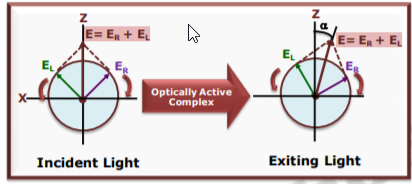
\includegraphics[width=0.8\textwidth]{Experiments/Polarimeter-fig1.png}
		\label{fig:polari-fig}
	\end{figure}
	
	It has been shown that since the speed of light in a medium is manifested in the refractive index of the medium, essential property of an optically active substance is that it has different refractive indices for the left and right circularly polarized light, nL and nR, respectively. This is also the reason why an optically active substance is said to be \textit{circularly birefringent}.
	
	{\textbf{Circular Birefringence}}: The difference in indices of refraction for right circularly polarized light (RCPL) and left circularly polarized light (LCPL) is known as circular birefringence. Thus, on passing plane polarized light (PPL) through optically active compound results in an unequal rate of propagation of right and left circularly polarized rays due to circular birefringence. This unequal rate of propagation for both right and left circularly polarized light deviate the PPL from its original direction and it is called \emph{optical rotation}. Optical rotation is caused by compound changes with the wavelength of PPL that means circular birefringence. Optical rotation is measured by polarimeter. Measuring optical rotation as a function of wavelength is termed as optical rotatory dispersion (ORD) spectroscopy. Circular birefringence or optical rotation can be calculated quantitatively by using the following equations:
	
	Angle of rotation $\phi$ per unit length expressed in $^{\circ}$ is given by
	\begin{equation}
		\label{eqn:Angle of rotation per unit length}
		\Phi=\frac{\pi}{\lambda}\left(n_{L}-n_{R}\right)
	\end{equation}
	where, $\lambda$ is the wavelength of incident light, $n_l$ and $n_R$ are the refractive indices for left and right circularly polarized light, and $l$ is the path length of the medium.
	
	Spectro polarimeters are the polarimeters used to make measurements at a variety of wavelength; they record `$\alpha$' as a function of $\lambda$ at a specific temperature. At a specified wavelength; optical rotation `$\alpha$' is called as specific rotation, $[\alpha]^{\mathrm{T}}_{\lambda}$, occasionally we use the term molar rotation $[\mathrm{M}]_{\lambda}$ Specific rotation, $[\alpha]_{\lambda}$ is given by:
	\begin{equation}
		[\alpha]_{\lambda}^{T}=\frac{\alpha}{l \times c}
	\end{equation}
	Where $\alpha$ is the observed rotation at wavelength $\lambda$ in degrees, 1 is the light path in decimeters, $\mathrm{c}$ is concentration of the optically active substance in grams per ml. For ORD we commonly we use molar rotation $[\mathrm{M}]_{\lambda}$ (unit: $^{\circ} \mathrm{cm}^{2} / \mathrm{dmol}$ ) which is defined as:
	$$
	[M]_{\lambda}=\frac{\alpha M}{100 l c}
	$$
	Where $\alpha$ is the observed rotation at wavelength $\lambda$ in degrees, 1 is the light path in decimeters, $\mathrm{c}$ is the concentration of the optically active substance in grams per $\mathrm{ml}$, and $\mathrm{M}$ is the molecular weight in grams per mol. A curve showing the wavelength dependence of optical rotation is called an Optical Rotatory Dispersion (ORD) spectrum. ORD curve is a plot of specific rotation, $[\alpha]$ vs $\lambda$ or molar rotation $[M]$ vs $\lambda$.
	
	
	
	
	\section{Procedure}
	
	\begin{enumerate}
		\item 	 Adjust the polarizer to get the direct beam of sodium/mercury light and note down its position.
		\item 	Place quartz crystal inside polarizer and note down the position where we find the uniform intensity throughout beam of vision.
		\item 	 Place colour filter in front of a source and rotate the polarizer so that you get the equal intensity of light throughout beam of vision.
		\item  	Calculate the background count by dividing the total number of counts by five.
		\item 	Note down  the angle through which it had  moved . 
		
		
		\item  	 Measure the thickness of quartz crystal using screw gauge
		
		
		\item 	Plot a graph between specific rotation and $\dfrac{1}{\lambda^2}$
		\item The slope will give the oscillator strength of the crystal. 
		
	\end{enumerate}
	
	\section{Observations \& Graph}
	
	
	
	The plot of Specific rotation  versus $ 1/\lambda^2 $ is shown in figure 
	\ref{fig:plot}.
	
	% 	\begin{figure}[!htb]
	% 		\centering
	% 		\includegraphics[width=0.8\textwidth]{Experiments/optical.png}
	% 		\caption{Plot of Specific rotation versus $ 1/\Lambda^2 $ }
	% 		\label{fig:plot}
	% 	\end{figure}
	
	\begin{table}[h]
		\begin{tabular}{|l|c|c|c|c|c|c|c|c|}
			\hline
			Filters & \multicolumn{1}{l|}{Wavelength (\AA)} & \multicolumn{4}{c|}{Position of crystal} & Avg Rotation & Specific Rotation & \multicolumn{1}{l|}{$\dfrac{1}{\lambda^2}$}\\ \hline
			Red     & 6230                                                       & 42       & 39       & 38       & 42      & 40.25        & 3003.73           & 2.576                                           \\ \hline
			Yellow  & 5780                                                       & 44       & 48       & 46       & 49      & 46.75        & 3488.8            & 2.993                                           \\ \hline
			Green   & 5461                                                       & 52       & 51       & 54       & 53      & 52.5         & 3917.91           & 3.353                                           \\ \hline
			Blue    & 4350                                                       & 61       & 59       & 63       & 62      & 61.25        & 4510.89           & 5.285                                           \\ \hline
		\end{tabular}
	\end{table}
	\clearpage
	\section{Result}
	The oscillator strength of quartz crystal is found to be \num{571.70 e-12}\ $m^3$
	
	%	\section{References}
	
\end{document}